\lesson{11}{May 14 2022 Sat (07:51:22)}{Right Triangle Trigonometry}

\begin{figure}[htpb]
	\centering

	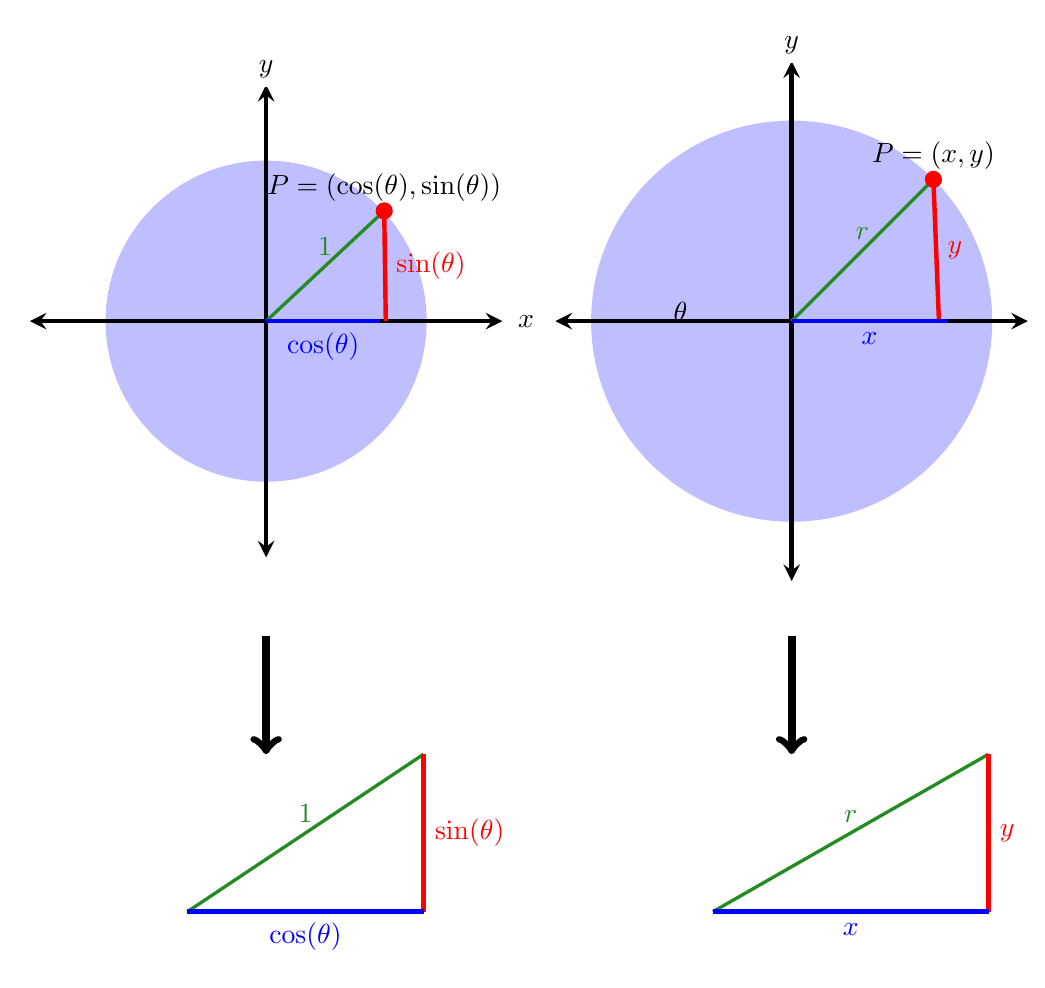
\begin{tikzpicture}
		% Smaller Circle
		\coordinate (origin) at (-5,0);
		\coordinate (x1) at (-8,0);
		\coordinate (x2) at (-2,0);
		\coordinate (y1) at (-5,-3);
		\coordinate (y2) at (-5,3);
		\coordinate (p) at (-3.5,1.4);
		\coordinate (P) at (p) ++(0.02,-0.05);
		\coordinate (arrow1) at (-5,-4);
		\coordinate (arrow2) at (-5,-5.5);
		\coordinate (sin1) at (-3.48,0);
		\coordinate (cos1) at (-3.55,0);

		\draw[draw=blue!25!white,fill=blue!25!white] (origin) circle (0.8in);
		\draw[stealth-stealth,ultra thick] (x1) -- (x2);
		\draw[stealth-stealth,ultra thick] (y1) -- (y2);
		\draw (y2) ++(0,0.2) node[fill=white,anchor=center] {$y$};
		\draw (x2) ++(0.3,0) node[fill=white,anchor=center] {$x$};
		\draw[ForestGreen,very thick] (origin) to node[anchor=south] {$1$} (p);
		\draw[draw=red,fill=red] (P) circle (0.04in);
		\draw (P) node[anchor=south] {$P = (\cos (\theta), \sin (\theta))$};
		\draw[ultra thick,red] (P) to node[anchor=west] {$\sin (\theta)$} (sin1);
		\draw[ultra thick,blue] (origin) to node[anchor=north] {$\cos (\theta)$} (cos1);

		% Smaller Triangle
		\draw[->, line width=1mm] (arrow1) -- (arrow2);
		\coordinate (a) at (-6,-7.5);
		\coordinate (b) at (-3,-5.5);
		\coordinate (c) at (-3,-7.5);
		\draw[ForestGreen,very thick] (-6,-7.5) to node[anchor=south] {$1$} (-3,-5.5);
		\draw[ultra thick,red] (-3,-5.5) to node[anchor=west] {$\sin (\theta)$} (-3,-7.5);
		\draw[ultra thick,blue] (-6,-7.5) to node[anchor=north] {$\cos (\theta)$} (-3,-7.5);
		\tkzMarkAngle[mark=none](c,a,b);
		\tkzLabelAngle[pos=0.6](c,a,b){$\theta$};

		% Bigger Circle
		\coordinate (origin) at (1.5,0);
		\coordinate (x1) at (4.5,0);
		\coordinate (x2) at (-1.5,0);
		\coordinate (y1) at (1.5,3.3);
		\coordinate (y2) at (1.5,-3.3);
		\coordinate (p) at (3.3,1.8);
		\coordinate (P) at (p) ++(0.02,0.05);
		\coordinate (arrow1) at (1.5,-4);
		\coordinate (arrow2) at (1.5,-5.5);
		\coordinate (x) at (3.48,0);
		\coordinate (y) at (3.37,0);

		\draw[draw=blue!25!white,fill=blue!25!white] (origin) circle (1in);
		\draw[stealth-stealth,ultra thick] (x1) -- (x2);
		\draw[stealth-stealth,ultra thick] (y1) -- (y2);
		\draw (y1) ++(0,0.2) node[fill=white,anchor=center] {$y$};
		\draw[ForestGreen,very thick] (origin) to node[anchor=south] {$r$} (p);
		\draw[draw=red,fill=red] (P) circle (0.04in);
		\draw (P) node[anchor=south] {$P = (x, y)$};
		\draw[ultra thick,red] (P) to node[anchor=west] {$y$} (y);
		\draw[ultra thick,blue] (origin) to node[anchor=north] {$x$} (x);

		% Bigger Triangle
		\draw[->, line width=1mm] (arrow1) -- (arrow2);
		\coordinate (a) at (0.5,-7.5);
		\coordinate (b) at (4,-5.5);
		\coordinate (c) at (4,-7.5);
		\draw[ForestGreen,very thick] (a) to node[anchor=south] {$r$} (b);
		\draw[ultra thick,red] (b) to node[anchor=west] {$y$} (c);
		\draw[ultra thick,blue] (a) to node[anchor=north] {$x$} (c);
		\tkzMarkAngle[mark=none](c,a,b);
		\tkzLabelAngle[pos=0.6](c,a,b){$\theta$};
	\end{tikzpicture}

	\caption{The angle of $\theta$ in both a unit circle and in a circle of radius
		$r$, including similar right triangles.}
	\label{fig:circle_to_triangle}
\end{figure}

We can use these triangles to create ratios.

\noindent\begin{minipage}{.33\linewidth}
	\begin{align*}
		\qquad         & \frac{\sin (\theta)}{1} = \frac{y}{r} \\
		\implies\qquad & \sin (\theta) = \frac{y}{r}           \\
	\end{align*}
\end{minipage}
\hfill\vline\hfill
\begin{minipage}{.33\linewidth}
	\begin{align*}
		\qquad         & \frac{\cos (\theta)}{1} = \frac{x}{r} \\
		\implies\qquad & \cos (\theta) = \frac{x}{r}           \\
	\end{align*}
\end{minipage}

\begin{figure}[htpb]
  \centering

  \begin{tikzpicture}
    \coordinate (a) at (0,0);
    \coordinate (b) at (4,0);
    \coordinate (c) at (4,4);
    \draw[ForestGreen] (a) -- (c);
    \draw[red] (c) -- (b);
    \draw[blue] (a) -- (b);
    \tkzLabelSegment (a,c) {$r$};
    \tkzLabelSegment (c,b) {$y$};
    \tkzLabelSegment (a,b) {$x$};

		\draw[->, line width=1mm] (5,2) -- (6,2);

    \coordinate (a) at (7,0);
    \coordinate (b) at (11,0);
    \coordinate (c) at (11,4);
    \draw[ForestGreen] (a) -- (c);
    \draw[red] (c) -- (b);
    \draw[blue] (a) -- (b);
    \tkzLabelSegment (a,c) {HYP};
    \tkzLabelSegment (c,b) {OPP};
    \tkzLabelSegment (a,b) {ADJ};
  \end{tikzpicture}

  \caption{We use the terms \textbf{opposite} (or \textbf{OPP}),
    \textrm{adjacent} (or \textbf{ADJ}), and \textbf{hypotenuse}
    (or \textbf{HYP}) to refer to the sides of a right triangle.}
  \label{fig:x_y_r_triangle_to_adj_opp_hyp_triangle}
\end{figure}

\newpage

\begin{definition}
  If $\theta$ is the angle given in the right triangles in Figure
  \ref{fig:x_y_r_triangle_to_adj_opp_hyp_triangle}, then
	\[
		\sin (\theta) = \frac{y}{r} =  \frac{\textrm{OPP}}{\textrm{HYP}}
		\qquad \cos (\theta) = \frac{x}{r} = \frac{\textrm{AJD}}{\textrm{HYP}}
		\qquad \tan (\theta) = \frac{y}{x} = \frac{\textrm{OPP}}{\textrm{ADJ}}
	\].

	Consequently, the other trigonometric functions can be defined as follows:
	\[
		\cot (\theta) = \frac{\textrm{ADJ}}{\textrm{OPP}}
		\qquad \sec (\theta) = \frac{\textrm{HYP}}{\textrm{ADJ}}
		\qquad \csc (\theta) = \frac{\textrm{HYP}}{\textrm{OPP}}
	\].

	There's a mnemonic that you can use to remember this:

	\begin{center}
		\textrm{SOH CAH TOA}
	\end{center}
\end{definition}

\begin{exc}[Solution \ref{sol:find_value_for_all_six_trigonometric_functions}]
  \label{exc:find_value_for_all_six_trigonometric_functions}

  Find the value for all six trigonometric functions of the angle $\alpha$ given
  in the right triangle in Figure \ref{fig:alpha_triangle}. (The triangle isn't
  drawn to scale)

  \begin{figure}[H]
    \centering

    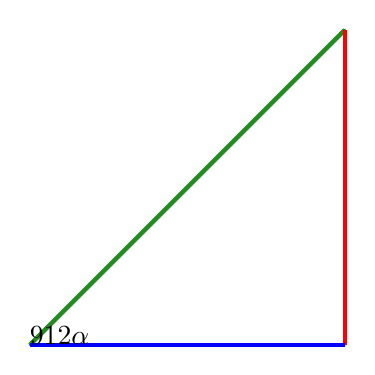
\begin{tikzpicture}
      \coordinate (a) at (0,0);
      \coordinate (b) at (4,0);
      \coordinate (c) at (4,4);

      \draw (a) -- (c) -- (b) -- cycle;

      \draw[ultra thick,ForestGreen] (a) -- (c);
      \draw[ultra thick,red] (c) -- (b);
      \draw[ultra thick,blue] (a) -- (b);

      \tkzLabelSegment (c,b) {$9$};
      \tkzLabelSegment (a,b) {$12$};
      \tkzMarkAngle[mark=none](b,a,c);
      \tkzLabelAngle[pos=0.6](b,a,c){$\alpha$};
    \end{tikzpicture}

    \caption{}
    \label{fig:alpha_triangle}
  \end{figure}
\end{exc}

We can use the trig functions, along with the Pythagorean Theorem to
\textbf{"solve a right triangle"}, i.e., find the missing side-lengths and
missing angle-measures for a triangle.

\begin{exc}[Solution \ref{sol:solving_a_right_triangle}]
  \label{exc:solving_a_right_triangle}

  Solve the right triangle given in Figure \ref{fig:solving_a_right_triangle} by
  finding $A$, $b$, and $c$. (The triangle may not be drawn to scale.)

  \begin{figure}[H]
    \centering

    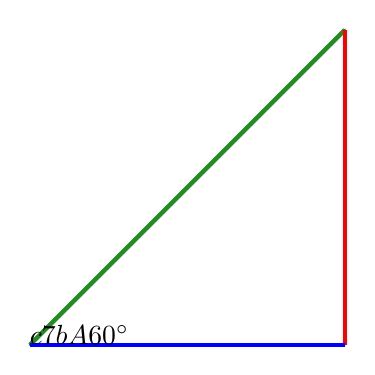
\begin{tikzpicture}
      \coordinate (a) at (0,0);
      \coordinate (b) at (4,0);
      \coordinate (c) at (4,4);

      \draw (a) -- (c) -- (b) -- cycle;

      \draw[ultra thick,ForestGreen] (a) -- (c);
      \draw[ultra thick,red] (c) -- (b);
      \draw[ultra thick,blue] (a) -- (b);

      \tkzLabelSegment (a,c) {$c$};
      \tkzLabelSegment (c,b) {$7$};
      \tkzLabelSegment (a,b) {$b$};
      \tkzMarkAngle[mark=none](b,a,c);
      \tkzMarkAngle[mark=none](a,c,b);
      \tkzLabelAngle[pos=0.6](b,a,c){$A$};
      \tkzLabelAngle[pos=0.6](a,c,b){$60^{\circ}$};
    \end{tikzpicture}

    \caption{}
    \label{fig:solving_a_right_triangle}
  \end{figure}
\end{exc}

\newpage
